\chapter{Validation \& Experiments}

In this chapter the validation of the algorithm is tested. This testing happens in three tests. Section \ref{sec:scenarios-testing} present the findings of a technical test in which test scenarios are designed to test the algorithm. It starts with setting up in memory graphs and assert the merge graph outcome. Section \ref{sec:experimental-application} shows the use of an external application the is tested by \testar. The external application is an experimental test application, in which it is possible to create three different versions. The last test is conducted using a real live application, tested by \testar. 

\todo{Create Last test}

% using login because it is be able to sign in immediately 
%\begin{verbatim*}
%"C:\tools\chromedriver.exe" "1920x900+0+0" "http://localhost:8100/Login"
%\end{verbatim*}

%To prevent the system to logout it is needed to filter the logout action, \verb|.*Logout.*| added to the filter option. 

%\begin{lstlisting}[language=Java, caption=Begin Sequence code, label=code:beginSequence]%
%@Override
%protected void beginSequence(SUT system, State state) {
%	%super.beginSequence(system, state);

%	waitLeftClickAndPasteIntoWidgetWithMatchingTag("id", "url", "http://localhost:5000", state, system, 5,1.0);
%	waitLeftClickAndTypeIntoWidgetWithMatchingTag("id","username", "testar2\\testar", state, system, 5,1.0);
%	waitLeftClickAndTypeIntoWidgetWithMatchingTag("id","password", "testar", state, system, 5,1.0);
%	waitAndLeftClickWidgetWithMatchingTag("name", "Sign In", state, system, 5, 1.0);
%}
%\end{lstlisting}

\newpage

\section{Gherkin style testing} \lable{sec:scenarios-testing}
The first form of validation the algorithm is done with Gherkin syntax testing. Gherkin is syntax that describes a test scenario. The syntax uses special keywords like \textbf{Given}, \textbf{When}, \textbf{Then} to describe a \textit{scenario}. An example of a Gherkin scenario can be found in listing \ref{code:gherkin-example}.

\begin{lstlisting}[language=Gherkin, caption=Calculator test example, label=code:gherkin-example]
Scenario: Add two numbers
Given the first number is 50
And the second number is 70
When the two numbers are added
Then the result should be 120
\end{lstlisting}

A developer can automated the Gherkin syntax to create automated test cases for example with the help of Specflow \footnote{\url{https://www.specflow.com}}. Specflow is a test automation solution for the .NET framework \cite{specflow}. The code to automate the 'then' line in listing \ref{code:gherkin-example} can be implemented as indicated in listing \ref{code:gherkin-example-code}.

\begin{lstlisting}[language=Java, caption=Implementation of a 'then' line, label=code:gherkin-example-code]
[Then("the result should be (.*)")]
public void ThenTheResultShouldBe(int expectedResult)
{
    Assert.AreEqual(expectedResult, actualResult);
}
\end{lstlisting}

To validate the algorithm and the merging of the two abstract models (see \ref{sec:merge-graph}) a couple of scenario are written. The scenario's can be found in appendix \ref{appendix:test-scenarios}. The file start with the keyword \textbf{Feature} which is Specflow solution to group scenario's together. The \textbf{Background} section generates four in-memory graphs. In figure \ref{fig:test-graphs} four graphs are visualised. 

\newpage
\begingroup
\captionsetup{type=figure}
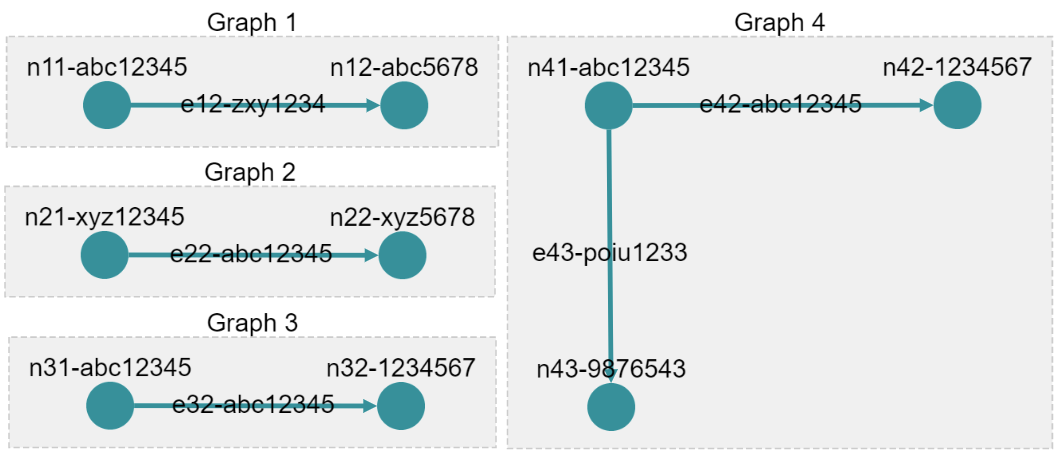
\includegraphics[scale=0.6]{images/6-TestGraphs.png}
\captionof{figure}{Test graphs used for testing. The circle represents a abstract state, the line represents the abstract actions between the abstract states}\label{fig:test-graphs}
\endgroup

Each scenario follows the same pattern, first two graphs from the background are chosen and set as either the old and new graphs. Then the comparison is run and the comparison result is merged. After the merge the actual result is asserted with the validation. Using the pattern five scenario were tested, divided in four specific tests and the fifth scenario being a bigger test representing an application of the experiment. See ... for more details about that experiment. 

\todo{Add more information about experiment}

The four specific tests are as follow: (1) validation that the initial states are recognised as corresponding states, (2) Going from an corresponding state, following an action with the same id, validate that the target state is recognised as corresponding states, (3) When a new abstract state is added validate it is recognised and merge as such, (4) When a abstract state is removed in the new version validate it is recognised and merged as such.

The fifth scenario used two different graphs, which are visualised in figure \ref{fig:bigger-test-graphs}. The graphs both has the same initial state, going to a middle state in which actions v1, v2 and v3 can be executed. In graph 6 the v3 action has been added and the v1 action is removed. By running the scenario a merge graph is generated which is visualised in figure \ref{fig:test-merged-graph}. The merge graph is exactly what was expected. 

\begingroup
\captionsetup{type=figure}
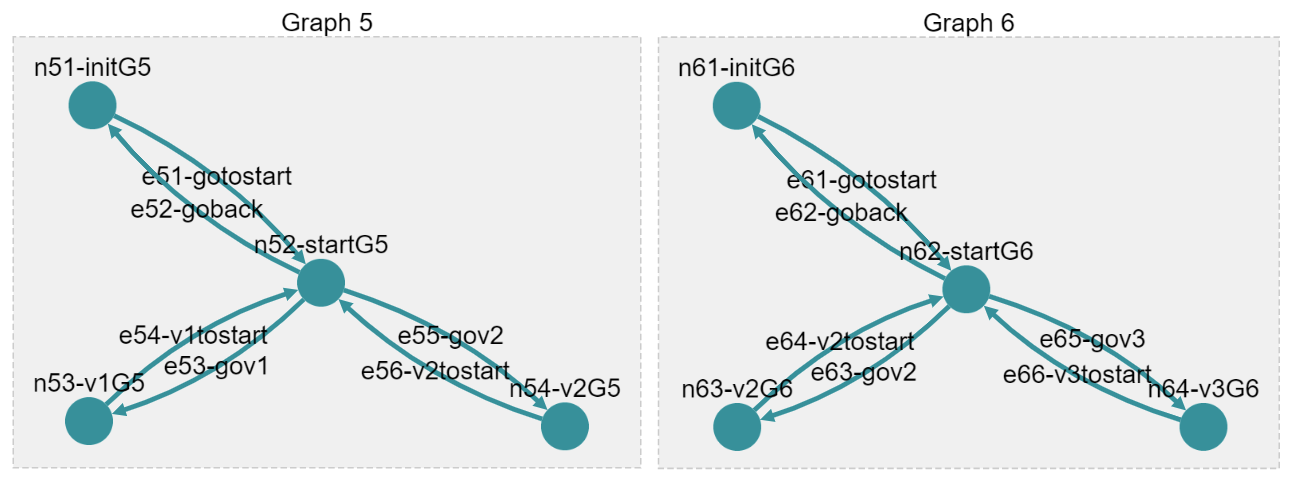
\includegraphics[scale=0.5]{images/6-test-graph-5-6.png}
\captionof{figure}{Graph 5 and 6 for bigger scenario. The circle represents a abstract state, the line represents the abstract actions between the abstract states}\label{fig:bigger-test-graphs}
\endgroup

In the merge graph are different shapes and colours visible. Red means a removed abstract state, but is also given a different shape in case of printing or for people which are colour blind. The new start has the form of a star. 

\begingroup
\captionsetup{type=figure}
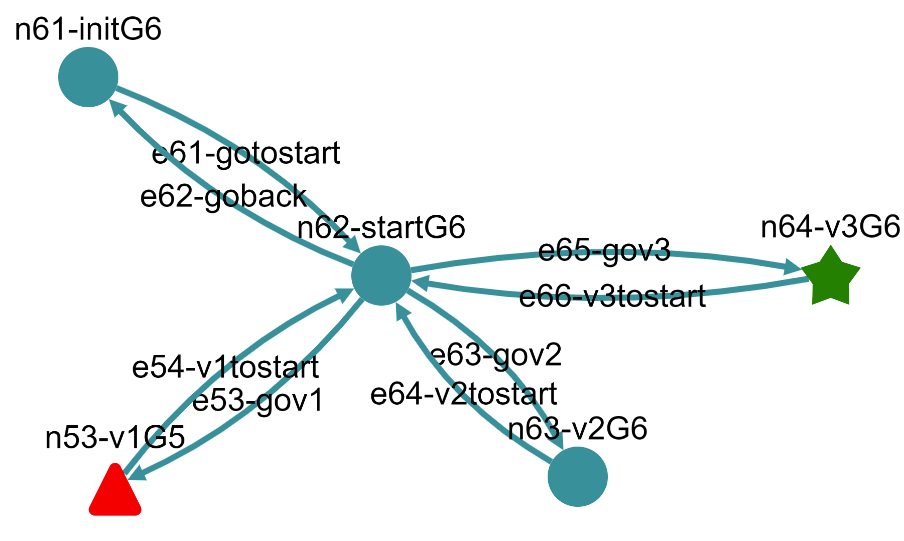
\includegraphics[scale=0.5]{images/6-merge-result.png}
\captionof{figure}{The merge result visualised. The circle represents a abstract state, a green star represents a new and the red triangle represents a removed abstract state, the line represents the abstract actions between the abstract states }\label{fig:test-merged-graph}
\endgroup


\subsubsection{Outcome}
By running the scenario's one issue was found in the merge engine. In section \ref{sec:merge-graph} under how to merge the graph is explained that the edged (abstract actions in \testar case) must be rewired from the old graph to the new graph. This was done but also for the actions that were already in the merge graph (which has the same action Ids). The led to duplication of edges. This issue is fixed by keeping track of action id in the merge graph. When a edge from the old graph contain an action id in the list than it is not rewired.

\section{Experimental application} \label{sec:experimental-application}

\subsection{The application}
The application under test is an application created in .NET. The source code can be found in the companion GitHub repository \footnote{}

